\documentclass{beamer}
\usepackage[latin1]{inputenc}
\usepackage{times}
\usepackage{tikz}
\usetheme{Luebeck}
%\usecolortheme{albatross}
\usepackage{amsmath,amsfonts,amsthm,amssymb}
\usepackage{setspace}
\usepackage{Tabbing}
\usepackage{fancyhdr}
\usepackage{lastpage}
\usepackage{extramarks}
\usepackage{chngpage}
\usepackage{soul,color}
\usepackage{graphicx,float,wrapfig}
\usepackage{xcolor}
\usepackage{listings}
\usepackage{float}
%\usepackage{subfloat}
\usepackage{subfig}
\usepackage{caption}
\usepackage{enumitem}
\usepackage{algpseudocode}

\definecolor{darkorange}{RGB}{240, 120, 0}
\definecolor{darkgreen}{RGB}{0, 128, 0}

\setbeamercolor{background canvas}{bg=white}
\setbeamercolor{frametitle}{fg=white, bg=darkorange}
\setbeamercolor{normal text}{bg=black,fg=black}
\setbeamercolor{structure}{bg=black, fg=darkorange}


\lstdefinestyle{customc}{
  belowcaptionskip=1\baselineskip,
  breaklines=true,
  frame=L,
  xleftmargin=\parindent,
  language=C,
  showstringspaces=false,
  basicstyle=\footnotesize\ttfamily,
  keywordstyle=\bfseries\color{green!40!black},
  commentstyle=\itshape\color{purple!40!black},
  identifierstyle=\color{blue},
  stringstyle=\color{orange},
}

\title{Lecture 13: Procrustes, ICP}
\date{2/25/2016}
\institute{Chris Tralie, Duke University}
\author{COMPSCI/MATH 290-04}
\begin{document}

\frame{\titlepage}

\begin{frame}{Announcements}
\begin{itemize}[label=$\vartriangleright$]

\item Group Assignment 1 Full Submission Due next Tuesday 11:55 PM

\item Hackathon Saturday 2/27 4:00 PM - 10:00 PM Gross Hall 330

\item Rank Top 3 Final Project Choices By Next Wednesday 3/2 (Groups of 3-4)

\end{itemize}

\end{frame}

\begin{frame}{Table of Contents}
\begin{itemize}[label=$\blacktriangleright$]
	\item Procrustes SVD Derivation
\end{itemize}
\begin{itemize}[label=$\vartriangleright$]
	\item ICP 
\end{itemize}
\end{frame}

\begin{frame}{Procrustes Rotation Problem}

Given correspondences, find best rotation

\begin{figure}[t]
	\centering
    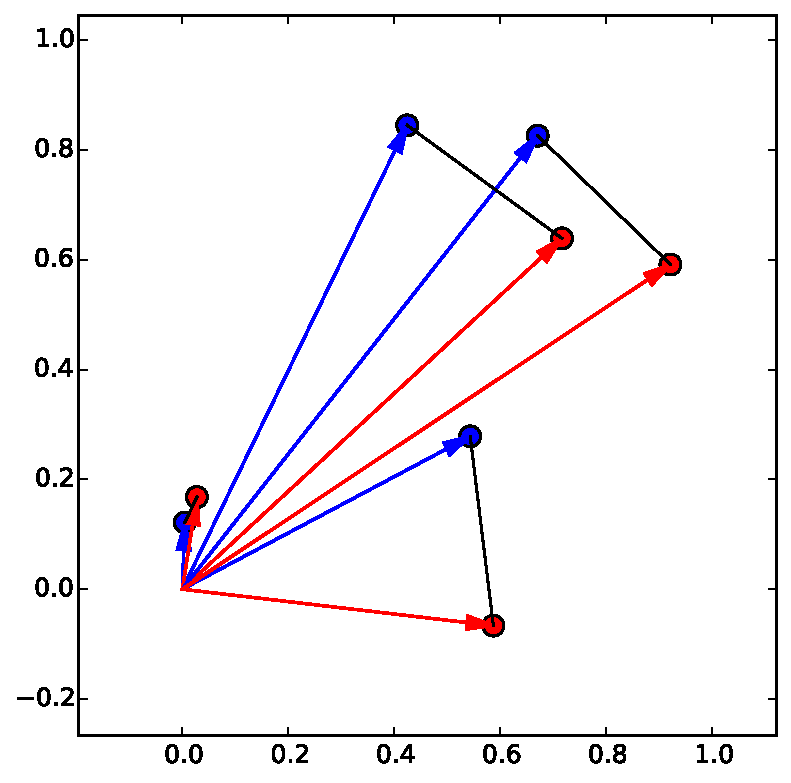
\includegraphics[width=0.5\textwidth]{2DProcrustes1.pdf}
\end{figure}



\end{frame}

\begin{frame}{Rotating to Align Points: Dot Product Perspective}

Points are well aligned if 

\[ \vec{x_1} \cdot \vec{y_1} = ||\vec{x_1}|| ||\vec{y_1}|| \cos(\theta) \]

is {\em maximized}

\begin{figure}[t]
	\centering
    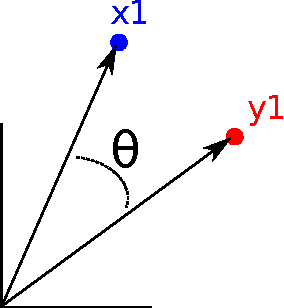
\includegraphics[width=0.4\textwidth]{PointsAlign.pdf}
\end{figure}

\end{frame}



\begin{frame}{Rotating to Align Points: Dot Product Perspective}

Points are well aligned if 

\[ \vec{x_1} \cdot \vec{y_1} = ||\vec{x_1}|| ||\vec{y_1}|| \cos(\theta) \]

is {\em maximized}

\begin{figure}[t]
	\centering
    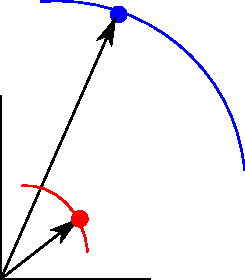
\includegraphics[width=0.4\textwidth]{PointsAlignArc.pdf}
\end{figure}

\end{frame}

\begin{frame}{Rotating to Align Points: Dot Product Perspective}

In general, how to maximize?

\[ \sum_{i = 1}^N \textcolor{blue}{R_x \vec{x_i}} \cdot \textcolor{red}{R_y \vec{y_i}} \]
\begin{figure}[t]
	\centering
    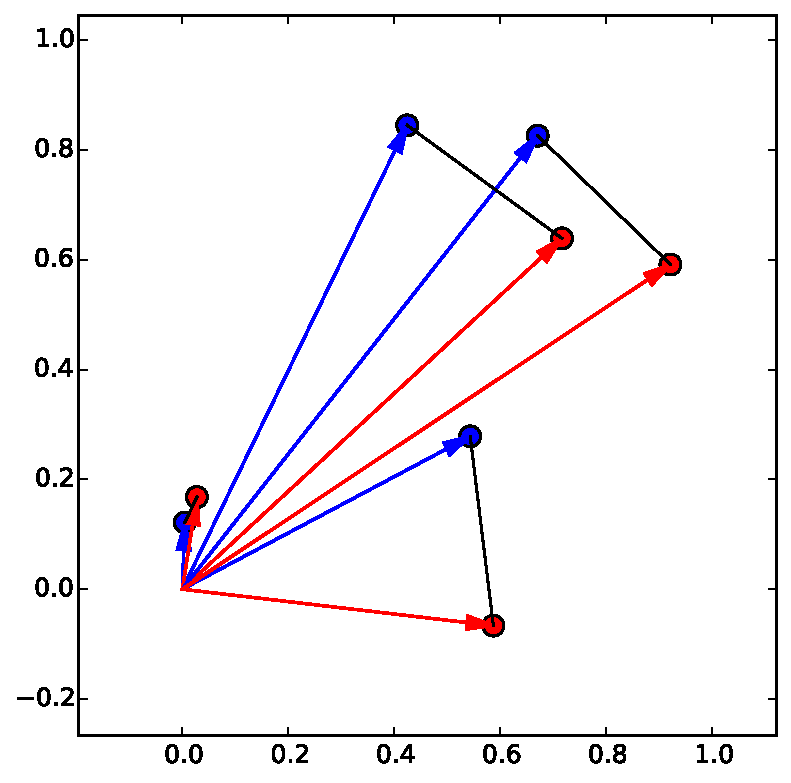
\includegraphics[width=0.5\textwidth]{2DProcrustes1.pdf}
\end{figure}


\end{frame}


\begin{frame}{Rotating to Align Points: Dot Product Perspective}

In general, how to maximize?

\[ \sum_{i = 1}^N \textcolor{blue}{R_x \vec{x_i}} \cdot \textcolor{red}{R_y \vec{y_i}} \]

VIDEO EXAMPLE


\end{frame}


\begin{frame}{Choosing Orthogonal Dot Product Axes}


\[ \sum_{i = 1}^N \textcolor{blue}{ \left[  \begin{array}{ccc} - & \vec{R_{x1}} & - \\ - & \vec{R_{x2}} & - \\ - & \vec{R_{x3}} & - \end{array} \right]  \left[ \begin{array}{c}  | \\ 
\vec{x_i} \\ |  \end{array} \right]  } \cdot \textcolor{red}{ \left[  \begin{array}{ccc} - & \vec{R_{y1}} & - \\ - & \vec{R_{y2}} & - \\ - & \vec{R_{y3}} & - \end{array} \right]  \left[ \begin{array}{c}  | \\ 
\vec{y_i} \\ |  \end{array} \right]   } \]

\begin{figure}[t]
	\centering
    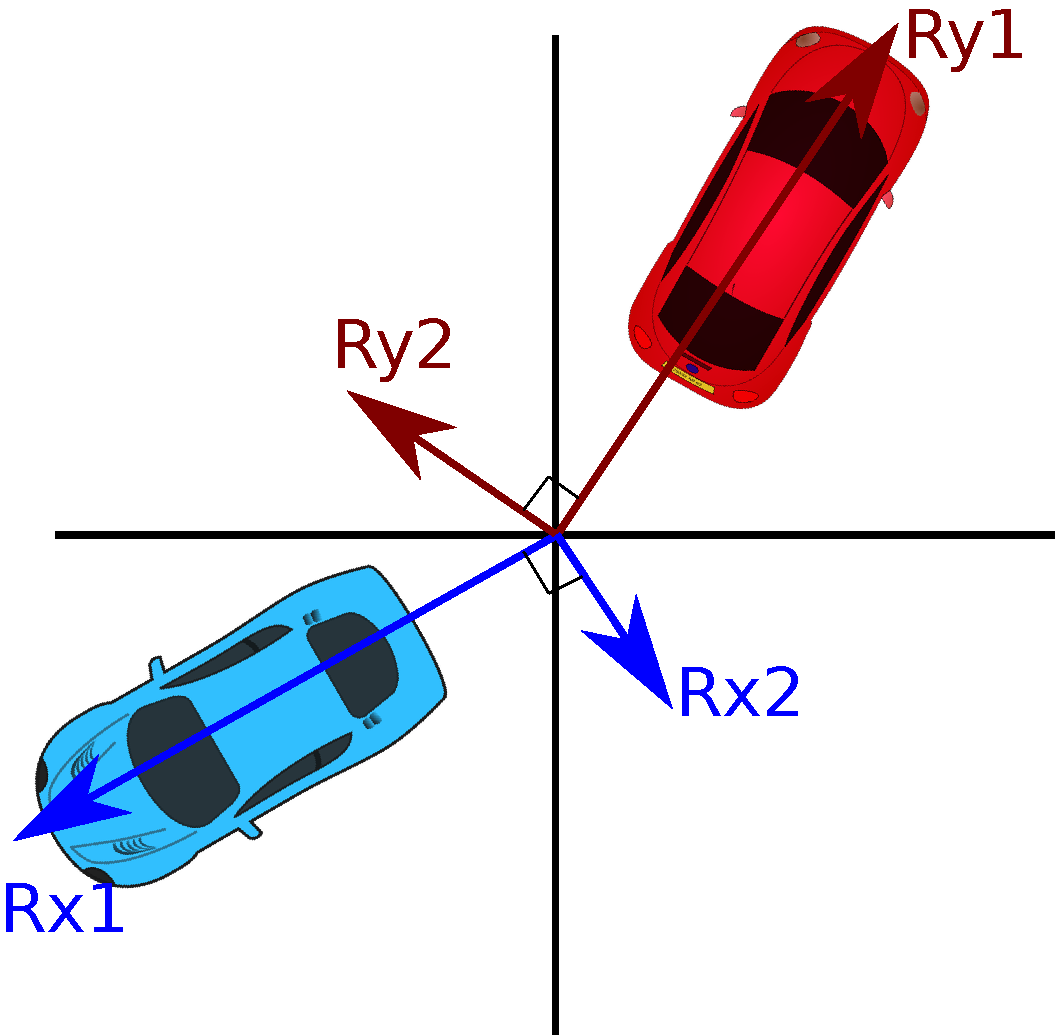
\includegraphics[width=0.56\textwidth]{CarsRotAxes.pdf}
\end{figure}


\end{frame}


\begin{frame}{Choosing Orthogonal Dot Product Axes}

\[ \sum_{i = 1}^N \textcolor{blue}{ \left[  \begin{array}{ccc} - & \vec{R_{x1}} & - \\ - & \vec{R_{x2}} & - \\ - & \vec{R_{x3}} & - \end{array} \right]  \left[ \begin{array}{c}  | \\ 
\vec{x_i} \\ |  \end{array} \right]  } \cdot \textcolor{red}{ \left[  \begin{array}{ccc} - & \vec{R_{y1}} & - \\ - & \vec{R_{y2}} & - \\ - & \vec{R_{y3}} & - \end{array} \right]  \left[ \begin{array}{c}  | \\ 
\vec{y_i} \\ |  \end{array} \right]   } \]

\[ = \]

\[ (\vec{R_{x1}} \cdot \vec{x_i})(\vec{R_{y1}} \cdot \vec{y_i}) + (\vec{R_{x2}} \cdot \vec{x_i})(\vec{R_{y2}} \cdot \vec{y_i}) + (\vec{R_{x3}} \cdot \vec{x_i})(\vec{R_{y3}} \cdot \vec{y_i})\]

\end{frame}

\begin{frame}{Maximizing Dot Product: First Component}

How to maximize $\sum_{i=1}^N  (\vec{R_{x1}} \cdot \vec{x_i})(\vec{R_{y1}} \cdot \vec{y_i})$?

\begin{figure}[t]
	\centering
    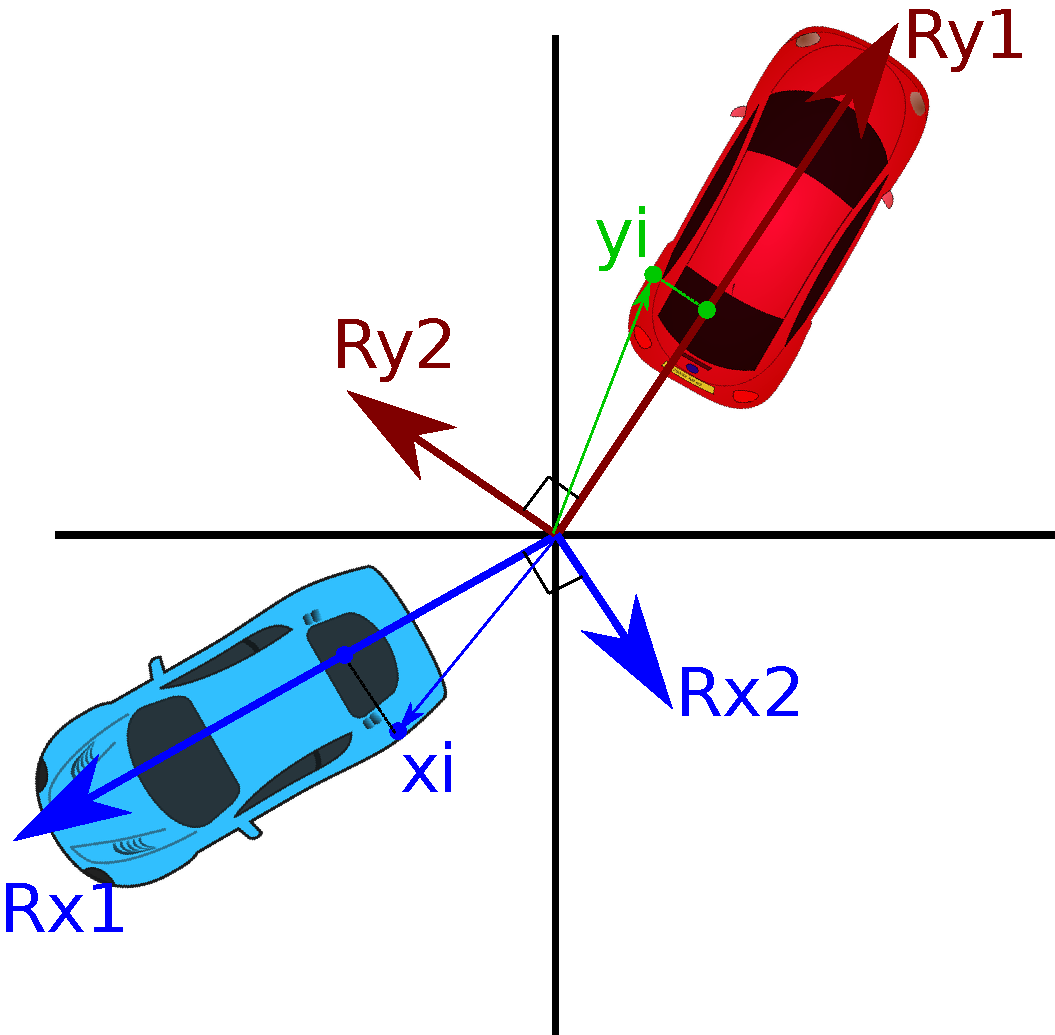
\includegraphics[width=0.56\textwidth]{CarRotAxesPointProj.pdf}
\end{figure}


\end{frame}


\begin{frame}{Maximizing Dot Product: First Component}

\[R_{x1} X, R_{y1} Y \]

How to write $\sum_{i=1}^N  (\vec{R_{x1}} \cdot \vec{x_i})(\vec{R_{y1}} \cdot \vec{y_i})$ in matrix form?

\uncover<2->{
\[  (R_{x1} X) (R_{y1} Y)^T = R_{x1} X Y^T R_{y1}^T \]
}

\begin{figure}[t]
	\centering
    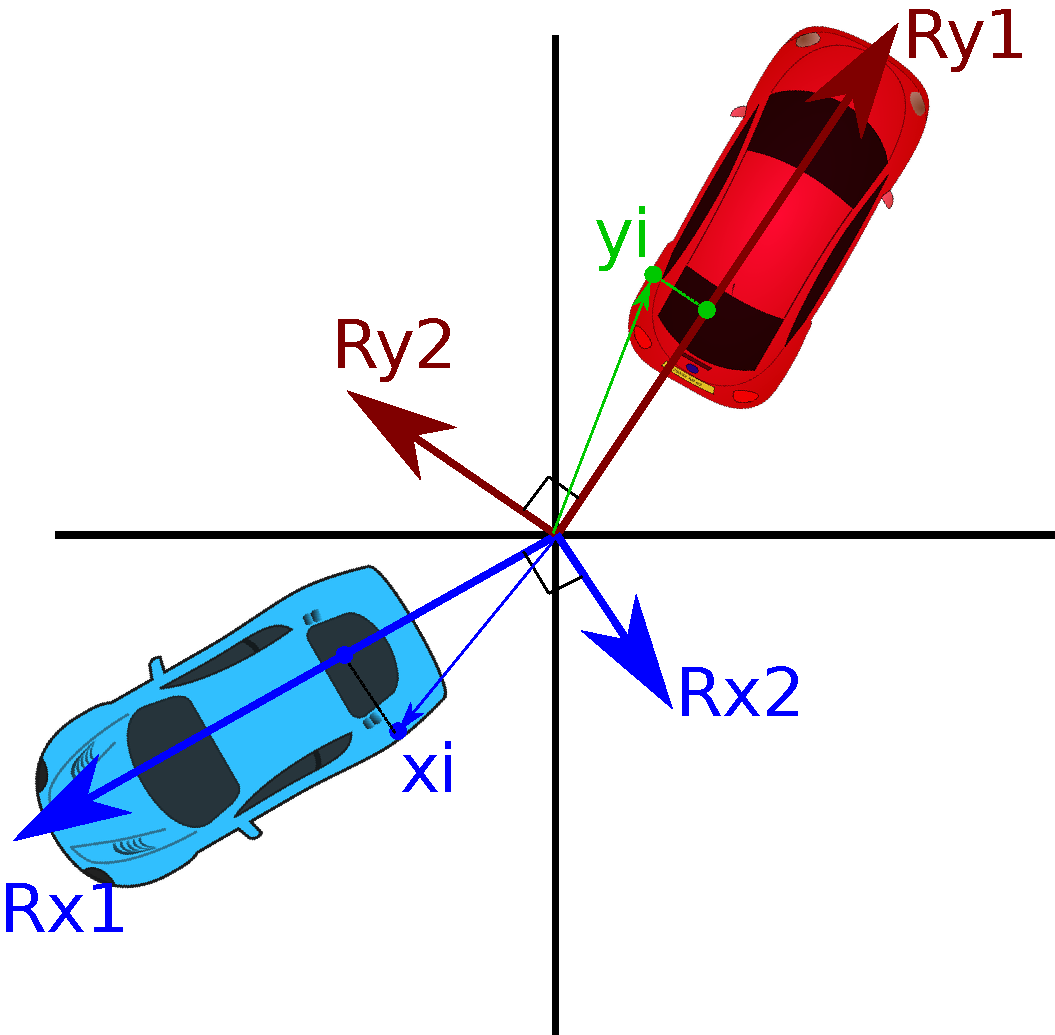
\includegraphics[width=0.4\textwidth]{CarRotAxesPointProj.pdf}
\end{figure}


\end{frame}


\begin{frame}{Maximizing Dot Product: First Component}

How to find $u_1$ and $v_1$ that maximize this product?

\[  (R_{x1} X) (R_{y1} Y)^T = R_{x1} X Y^T R_{y1}^T \]

Take SVD: $XY^T = USV^T$ and substitute in

\[ R_{x1} U S V^T R_{y1}^T \]


\end{frame}


\begin{frame}{Maximizing Dot Product: First Component}

\[ R_{x1} U S V^T R_{y1}^T \]

\small
\[ \left[ \begin{array}{ccc}-&\vec{R_{x1}}&-\end{array} \right] \left[ \begin{array}{ccc} | & | & | \\ \vec{u_1} & \vec{u_2} & \vec{u_3} \\ | & | & | \end{array} \right]  \left[ \begin{array}{ccc} s_1 & 0 & 0 \\ 0 & s_2 & 0 \\ 0 & 0 & s_3 \end{array} \right] \left[ \begin{array}{ccc} - & \vec{v_1} & - \\ - & \vec{v_2} & - \\ - & \vec{v_3} & - \end{array} \right] \left[ \begin{array}{c} | \\ \vec{R_{y1}} \\ | \end{array} \right] \]

Assume $s_1 > s_2 > s_3$, remember that $U$ and $V$ are orthogonal

\uncover<2->{
Raffle point question: Choose $\vec{R_{x1}}$ and $\vec{R_{y1}}$ to maximize this component of the dot product
}

\end{frame}

\begin{frame}{Maximizing Dot Product: First Component}
\[ R_{x1} U S V^T R_{y1}^T \]

\small
\[ \left[ \begin{array}{ccc} - & \vec{R_{x1}} & - \end{array} \right] \left[ \begin{array}{ccc} | & | & | \\ \vec{u_1} & \vec{u_2} & \vec{u_3} \\ | & | & | \end{array} \right]  \left[ \begin{array}{ccc} s_1 & 0 & 0 \\ 0 & s_2 & 0 \\ 0 & 0 & s_3 \end{array} \right] \left[ \begin{array}{ccc} - & \vec{v_1} & - \\ - & \vec{v_2} & - \\ - & \vec{v_3} & - \end{array} \right] \left[ \begin{array}{c} | \\ \vec{R_{y1}} \\ | \end{array} \right] \]

Assume $s_1 > s_2 > s_3$

\[ \vec{R_{x1}} = \vec{u_1}, \vec{R_{y1}} = \vec{v_1} \]

In other words

\begin{itemize}[label=$\vartriangleright$]
\item First row of $R_x$ is first column of $U$
\item First row of $R_y$ is first column of $V$
\end{itemize}

\end{frame}


\begin{frame}{Maximizing Dot Product: Second Component}

What about the second rows of $R_x$ and $R_y$ for second component of dot product?

\[ R_{x1} U S V^T R_{y1}^T \]

\[ R_{x2} U S V^T R_{y2}^T \]

\small
\[ \left[ \begin{array}{ccc} - & \vec{R_{x2}} & - \end{array} \right] \left[ \begin{array}{ccc} | & | & | \\ \vec{u_1} & \vec{u_2} & \vec{u_3} \\ | & | & | \end{array} \right]  \left[ \begin{array}{ccc} s_1 & 0 & 0 \\ 0 & s_2 & 0 \\ 0 & 0 & s_3 \end{array} \right] \left[ \begin{array}{ccc} - & \vec{v_1} & - \\ - & \vec{v_2} & - \\ - & \vec{v_3} & - \end{array} \right] \left[ \begin{array}{c} | \\ \vec{R_{y2}} \\ | \end{array} \right] \]

Assume $s_1 > s_2 > s_3$



\[ \sum_{i=1}^N  (\vec{R_{x1}} \cdot \vec{x_i})(\vec{R_{y1}} \cdot \vec{y_i}) \]

\end{frame}


\begin{frame}{Maximizing Dot Product: Full Rotation Matrix}



\tiny
\[ \textcolor{blue}{\left[ \begin{array}{ccc} - & \vec{u_1} & - \\ - & \vec{u_2} & - \\ - & \vec{u_3} & - \end{array} \right]} \left[ \begin{array}{ccc} | & | & | \\ \vec{u_1} & \vec{u_2} & \vec{u_3} \\ | & | & | \end{array} \right]  \left[ \begin{array}{ccc} s_1 & 0 & 0 \\ 0 & s_2 & 0 \\ 0 & 0 & s_3 \end{array} \right] \left[ \begin{array}{ccc} - & \vec{v_1} & - \\ - & \vec{v_2} & - \\ - & \vec{v_3} & - \end{array} \right] \textcolor{red}{\left[ \begin{array}{ccc} | & | & | \\ \vec{v_1} & \vec{v_2} & \vec{v_3} \\ | & | & | \end{array} \right]} \]

\small

\[ \textcolor{blue}{R_x} U S V^T \textcolor{red}{R_y^T} \]

Assume $s_1 > s_2 > s_3$

\begin{itemize}[label=$\blacktriangleright$]
\item Final answer for optimal rotations: $ R_x = U^T, R^y = V^T$
(Carefully working with transposes)
\end{itemize}

\end{frame}

\begin{frame}{Maximizing Dot Product: Full Rotation Matrix}

\begin{itemize}[label=$\blacktriangleright$]
\item Final answer for optimal rotations: $ R_x = U^T, R^y = V^T$
\end{itemize}

What if I want to just rotate $Y$ and keep $X$ fixed?  What should $R_y$ be?

\uncover<2->{
\[ R_y = UV^T \]

This is just SVD of $XY^T$ without $S$ !
}

\end{frame}

\begin{frame}{Enforcing Right Handedness}


\[ \left[ \begin{array}{ccc} - & \vec{u_1} & - \\ - & \vec{u_2} & - \\ - & \vec{u_3} & - \end{array} \right] \left[ \begin{array}{ccc} | & | & | \\ \vec{u_1} & \vec{u_2} & \pm \vec{u_3} \\ | & | & | \end{array} \right]  \left[ \begin{array}{ccc} s_1 & 0 & 0 \\ 0 & s_2 & 0 \\ 0 & 0 & s_3 \end{array} \right] \left[ \begin{array}{ccc} - & \vec{v_1} & - \\ - & \vec{v_2} & - \\ - & \vec{v_3} & - \end{array} \right] \left[ \begin{array}{ccc} | & | & | \\ \vec{v_1} & \vec{v_2} & \vec{v_3} \\ | & | & | \end{array} \right] \]


\small
Check if $\vec{u_1} \times \vec{u_2} = \vec{u_3}$.  If not, switch the sign of $\vec{u_3}$.  This subtracts from the function we're trying to maximize, but it does the minimal damage since $s_3 < s_2 < s_1$

\end{frame}


\begin{frame}{Rotation to Align Points: Algebra}
\[ \sum_{i=1}^N ||R\vec{x_i} - \vec{y_i}||_2^2 \]

How is this the same thing as maximizing sum of dot products?

\[ ||R\vec{x} - \vec{y}||^2 = (R\vec{x} - \vec{y}) \cdot (R\vec{x} - \vec{y}) \]


\uncover<2->{
\[  (R\vec{x} - \vec{y}) \cdot (R\vec{x} - \vec{y}) = R\vec{x} \cdot R\vec{x} + \vec{y} \cdot \vec{y} - 2 R\vec{x} \cdot \vec{y} \]
}

\uncover<3->{
\[  (R\vec{x} - \vec{y}) \cdot (R\vec{x} - \vec{y}) = ||R\vec{x}||^2 + ||\vec{y}||^2 - 2 R\vec{x} \cdot \vec{y} \]

}

\end{frame}


\begin{frame}{Procrustes Application: Moving Head Alignment}

VIDEO DEMO

\begin{figure}[t]
	\centering
    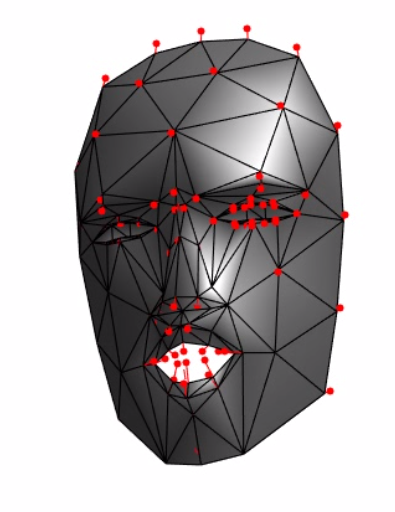
\includegraphics[width=0.4\textwidth]{MeProcrustes.png}
\end{figure}

\end{frame}


\begin{frame}{Procrustes Application: Average Faces}

Average Spaniards

\begin{figure}[t]
\centering
  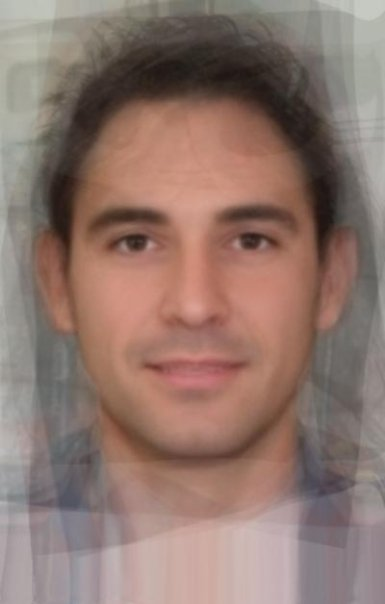
\includegraphics[width=0.4\textwidth]{averagespaniardmale.jpg}%
\end{figure}

\tiny \url{https://pmsol3.wordpress.com/2011/04/07/world-of-averages-europeave/}

\end{frame}

\begin{frame}{Procrustes Application: Average Faces}

Average Spaniards

\begin{figure}[t]
\centering
    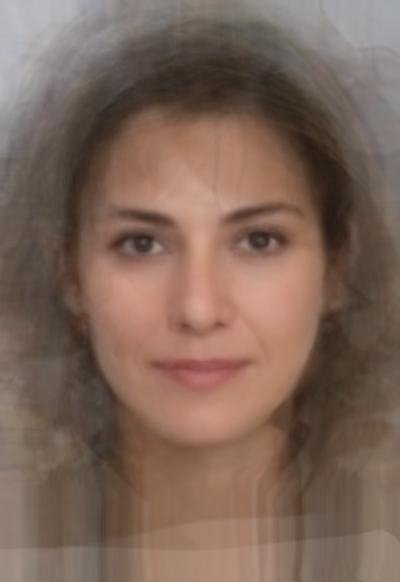
\includegraphics[width=0.4\textwidth]{averagespaniardfemale.jpg}%
\end{figure}

\tiny \url{https://pmsol3.wordpress.com/2011/04/07/world-of-averages-europeave/}

\end{frame}


\begin{frame}{Table of Contents}
\begin{itemize}[label=$\vartriangleright$]
	\item Procrustes SVD Derivation
\end{itemize}
\begin{itemize}[label=$\blacktriangleright$]
	\item ICP 
\end{itemize}
\end{frame}


\begin{frame}{ICP}


\begin{figure}[t]
	\centering
    
\includegraphics[width=0.6\textwidth]{icp.png}
\end{figure}


\end{frame}


\begin{frame}{ICP Example}

\begin{itemize}[label=$\vartriangleright$]
\item Iterative Closest Points
\item Iterative Closest Pairs
\item Iterative Corresponding Points
\end{itemize}

Goal: Automatically align two point sets

\begin{figure}[t]
\centering
    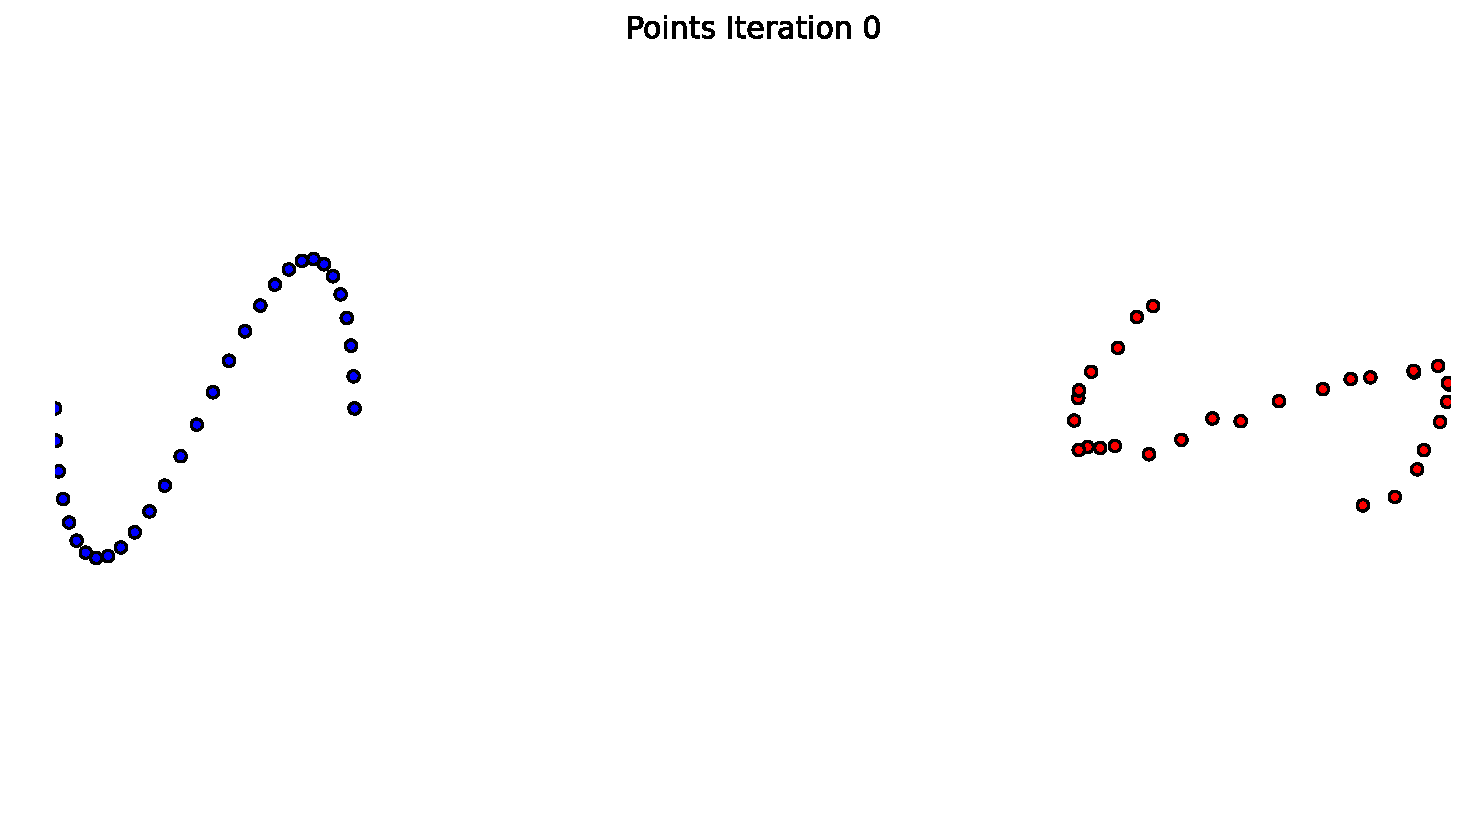
\includegraphics[width=\textwidth]{ICPExample/ICP0_1.pdf}%
\end{figure}


\end{frame}


\begin{frame}{ICP Example}

First mean center, now how to find correspondences automatically?

\begin{figure}[t]
\centering
    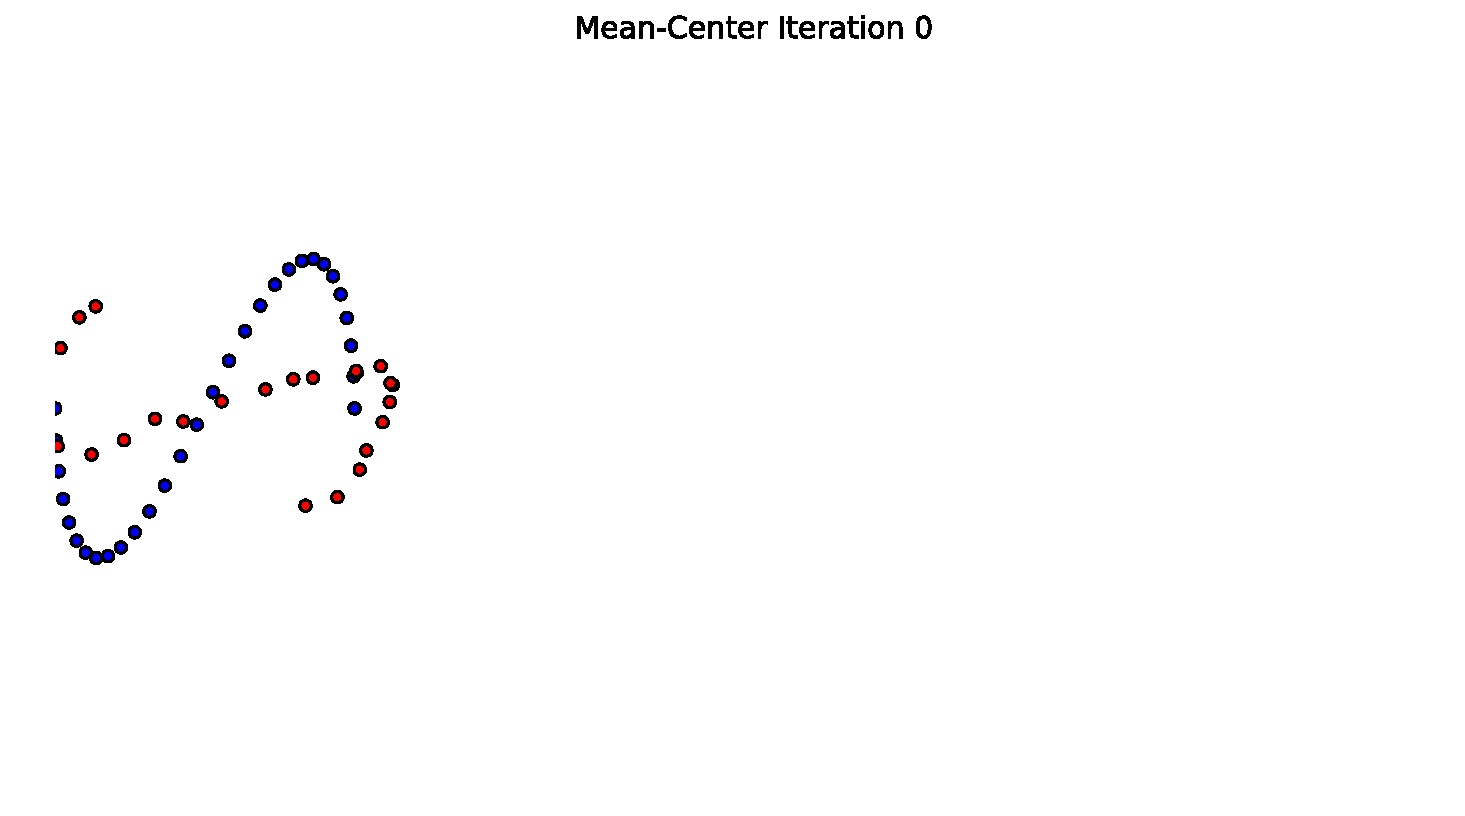
\includegraphics[width=\textwidth]{ICPExample/ICP0_2.pdf}%
\end{figure}


\end{frame}


\begin{frame}{ICP Example}

Use Nearest Neighbor, then do procrustes with those correspondences

\begin{figure}[t]
\centering
    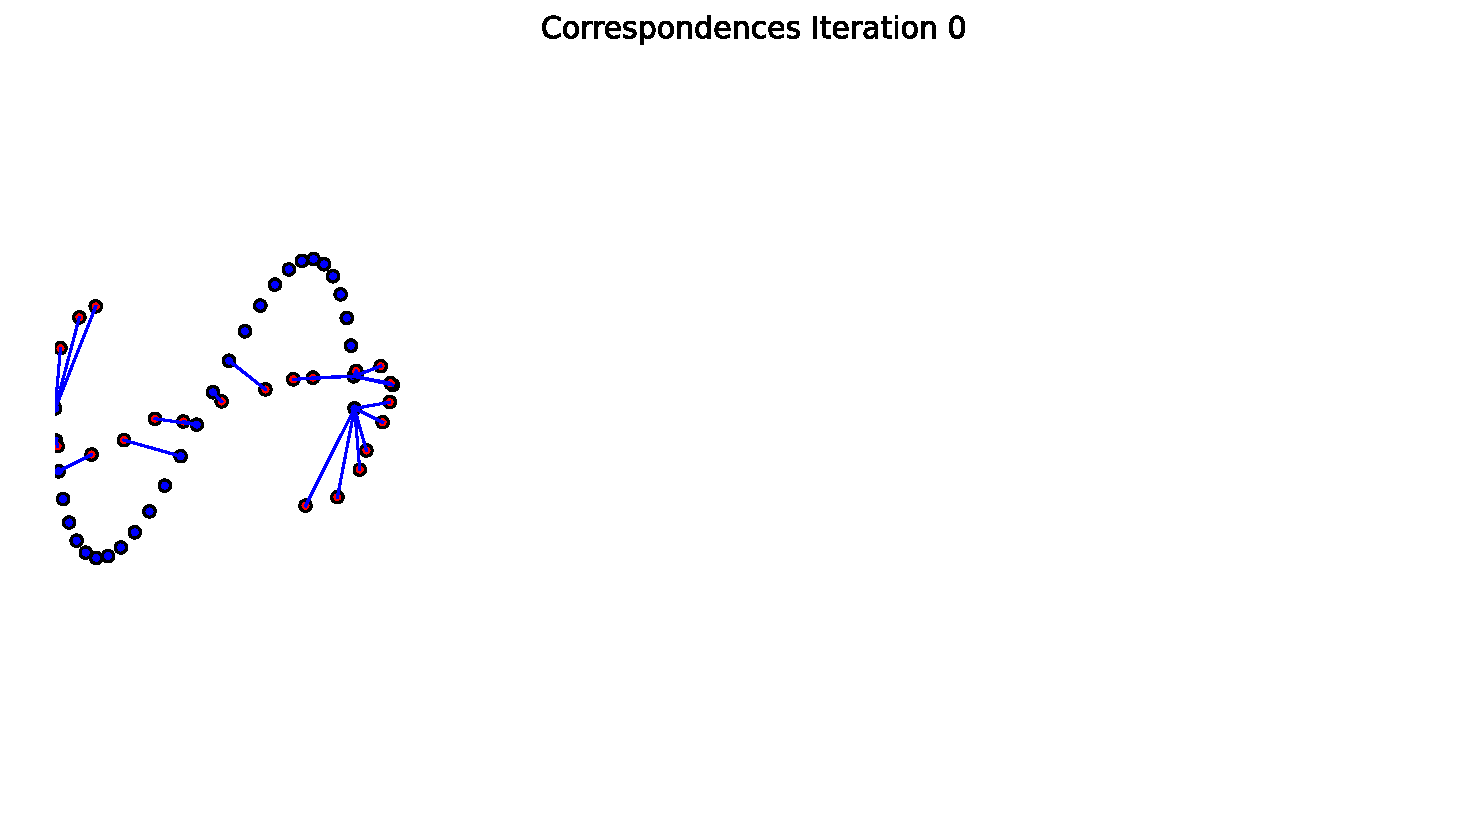
\includegraphics[width=\textwidth]{ICPExample/ICP0_3.pdf}%
\end{figure}

Some blue points may be duplicated!

\end{frame}


\begin{frame}{ICP Example}

Use Nearest Neighbor, then do procrustes with those correspondences

\begin{figure}[t]
\centering
    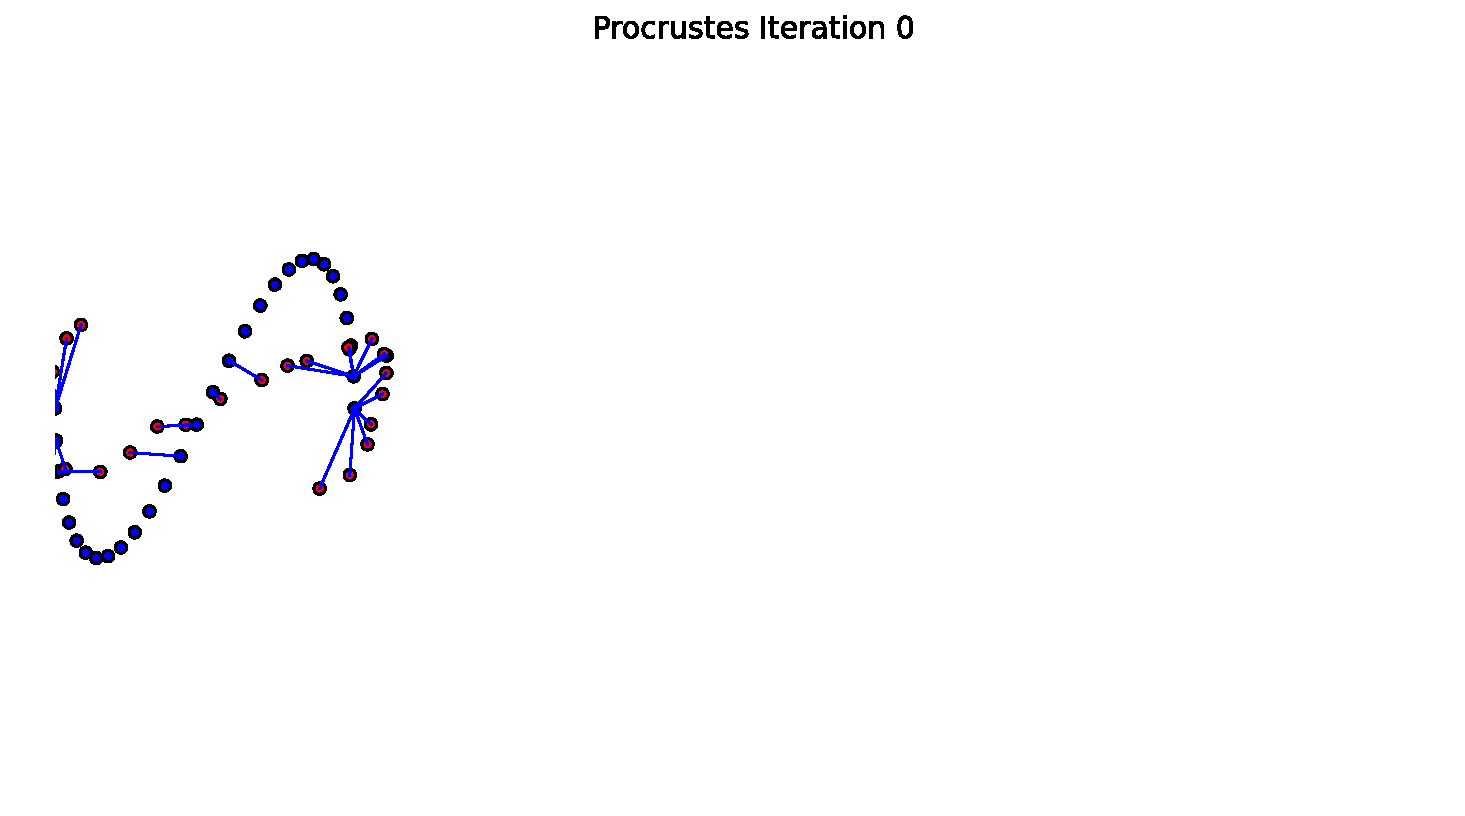
\includegraphics[width=\textwidth]{ICPExample/ICP0_4.pdf}%
\end{figure}

Some points may be repeated!

\end{frame}


\begin{frame}{ICP Example}

Continue, interactive...

\end{frame}


\begin{frame}{ICP Computation}

Steps in ICP Loop

\begin{itemize}

\item 1. Find nearest neighbors

\item 2. Procrustes rotation matrix

\item 3. Rotate Y Points, go back to step 1

\end{itemize}

For $N$ points in $X$ and $Y$, what is time complexity of each step?

\end{frame}


\begin{frame}{ICP Examples / Pitfalls}

Video Examples

\end{frame}

\begin{frame}{Final Projects}
Choices
\begin{itemize}
\item 1. Equidecomposing polygon meshes into each other in 3D, with SLERP animation
\item 2. Ghissi Alterpiece: Real Time Rendering Effects for NC Museum of Art
\item 3. Nasher Muesum Brummer Statue Heads Speech Transfer
\item 4. MOCAP Data Animation in Browser / Skinning / 3D Lemur Tracking(?)
\item 5. 3D Face Verification
\end{itemize}


OR

\begin{itemize}
\item 6. Individual project with approval
\end{itemize}

\end{frame}

\end{document}

